
%{{第五十八回}}{第五十八回}}

\chapter{杏子阴假凤泣虚凰\hspace{.5em}茜纱窗真情揆痴理}

{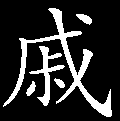
\includegraphics[width=3mm]{../Images/00005}  \kaishu 用清明烧纸徐徐引入园内烧纸,较之前文用燕窝隔回照应,别有草蛇灰线之趣,令人不觉。前文一接,怪蛇出水;此文一引,春云吐岫。}

话说他三人因见探春等进来,忙将此话掩住不提。探春等问候过,大家说笑了一会方散。

谁知上回所表的那位老太妃已薨,凡诰命等皆入朝随班按爵守制。敕谕天下:凡有爵之家,一年内不得筵宴音乐,庶民皆三月不得婚嫁。贾母、邢、王、尤、许婆媳祖孙等皆每日入朝随祭,至未正以后方回。在大内偏宫二十一日后,方请灵入先陵,地名曰孝慈县。{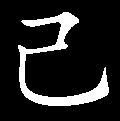
\includegraphics[width=3mm]{../Images/00003}随事命名。}这陵离都来往得十来日之功,如今请灵至此,还要停放数日,方入地宫,故得一月光景。{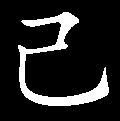
\includegraphics[width=3mm]{../Images/00003}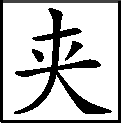
\includegraphics[width=3mm]{../Images/00012}\footnotesize \kaishu 周到细腻之至。◇真细之至,不独写侯府得理,亦且将皇宫赫赫,写得令人不敢坐阅。}宁府贾珍夫妻二人,也少不得是要去的。两府无人,因此大家计议,{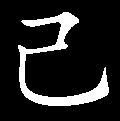
\includegraphics[width=3mm]{../Images/00003}家中无主,少不得又``大家计议''。}便报了尤氏产育,将他腾挪出来,协理荣宁两处事体。因又托了薛姨妈在园内照管他姊妹丫鬟。薛姨妈只得也挪进园来。因宝钗处有湘云香菱;李纨处目今李婶母女虽去,然有时亦来住三五日不定,贾母又将宝琴送与他去照管;迎春处有岫烟;探春因家务冗杂,且不时有赵姨娘与贾环来嘈聒,甚不方便;惜春处房屋狭小;况贾母又千叮咛万嘱咐托他照管林黛玉,薛姨妈素习也最怜爱他的,今既巧遇这事,便挪至潇湘馆来和黛玉同房,一应药饵饮食十分经心。黛玉感戴不尽,以后便亦如宝钗之呼,连宝钗前亦直以姐姐呼之,宝琴前直以妹妹呼之,俨似同胞共出,较诸人更似亲切。贾母见如此,也十分喜悦放心。薛姨妈只不过照管他姊妹,禁约得丫头辈,一应家中大小事务也不肯多口。尤氏虽天天过来,也不过应名点卯,亦不肯乱作威福,且他家内上下也只剩他一个料理,再者每日还要照管贾母王夫人的下处一应所需饮馔铺设之物,所以也甚操劳。

当下荣宁两处主人既如此不暇,并两处执事人等,或有人跟随入朝的,或有朝外照理下处事务的,又有先踩踏下处的,也都各各忙乱。因此两处下人无了正经头绪,也都偷安,或乘隙结党,与权暂执事者窃弄威福。荣府只留得赖大并几个管事照管外务。这赖大手下常用几个人已去,虽另委人,都是些生的,只觉不顺手。且他们无知,或赚骗无节,或呈告无据,或举荐无因,种种不善,在在生事,也难备述。

又见各官宦家,凡养优伶男女者,一概蠲免遣发,尤氏等便议定,待王夫人回家,回明也欲遣发十二个女孩子,又说:``这些人原是买的,如今虽不学唱,尽可留着使唤,令其教习们自去也罢了。''王夫人因说:``这学戏的倒比不得使唤的,他们也是好人家的儿女,因无能卖了做这事,装丑弄鬼的几年。如今有这机会,不如给他们几两银子盘费,各自去罢。当日祖宗手里都是有这例的。咱们如今损阴坏德,而且还小器。如今虽有几个老的还在,那是他们各有原故,不肯回去的,所以才留下使唤,大了配了咱们家的小厮们了。''尤氏道:``如今我们也去问他十二个,有愿意回去的,就带了信儿,叫上父母来,亲自来领回去,给他们几两银子盘缠方妥。若不叫上他父母亲人来,只怕有混账人顶名冒领出去又转卖了,岂不辜负了这恩典。若有不愿意回去的,就留下。''王夫人笑道:``这话妥当。''

尤氏等又遣人告诉了凤姐儿。{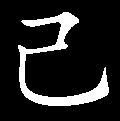
\includegraphics[width=3mm]{../Images/00003}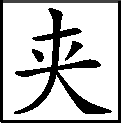
\includegraphics[width=3mm]{../Images/00012}\footnotesize \kaishu 看他任意鄙俚诙谐之中,必有一个``礼''字还清,足见是大家形景。}一面说与总理房中,每教习给银八两,令其自便。凡梨香院一应物件,查清注册收明,派人上夜。将十二个女孩子叫来面问,倒有一多半不愿意回家的:也有说父母虽有,他只以卖我们为事,这一去还被他卖了;也有父母已亡,或被叔伯兄弟所卖的;也有说无人可投的;也有说恋恩不舍的。所愿去者止四五人。王夫人听了,只得留下。将去者四五人皆令其干娘领回家去,单等他亲父母来领;将不愿去者分散在园中使唤。贾母便留下文官自使,将正旦芳官指与宝玉,将小旦蕊官送了宝钗,将小生藕官指与了黛玉,将大花面葵官送了湘云,将小花面荳官送了宝琴,将老外艾官送了探春,尤氏便讨了老旦茄官去。当下各得其所,就如倦鸟出笼,每日园中游戏。众人皆知他们不能针黹,不惯使用,皆不大责备。其中或有一二个知事的,愁将来无应时之技,亦将本技丢开,便学起针黹纺绩女工诸务。

一日正是朝中大祭,贾母等五更便去了,先到下处用些点心小食,然后入朝。早膳已毕,方退至下处,用过早饭,略歇片刻,复入朝待中晚二祭完毕,方出至下处歇息,用过晚饭方回家。可巧这下处乃是一个大官的家庙,乃比丘尼焚修,房舍极多极净。东西二院,荣府便赁了东院,北静王府便赁了西院。太妃少妃每日宴息,见贾母等在东院,彼此同出同入,都有照应。外面细事不消细述。

且说大观园中,因贾母王夫人天天不在家内,又送灵去一月方回,各丫鬟婆子皆有闲空,多在园内游玩。更又将梨香院内伏侍的众婆子一概撤回,并散在园内听使,更觉园内人多了几十个。因文官等一干人或心性高傲,或倚势凌下,或拣衣挑食,或口角锋芒,大概不安分守理者多。因此众婆子无不含怨,只是口中不敢与他们分证。如今散了学,大家称了愿,也有丢开手的,也有心地狭窄犹怀旧怨的,因将众人皆分在各房名下,不敢来厮侵。

可巧这日乃是清明之日,贾琏已备下年例祭祀,带领贾环、贾琮、贾兰三人去往铁槛寺祭柩烧纸。宁府贾蓉也同族中几人各办祭祀前往。因宝玉未大愈,故不曾去得。饭后发倦,袭人因说:``天气甚好,你且出去逛逛,省得丢下粥碗就睡,存在心里。''宝玉听说,只得拄了一支杖,靸着鞋,步出院外。{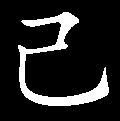
\includegraphics[width=3mm]{../Images/00003}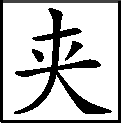
\includegraphics[width=3mm]{../Images/00012}\footnotesize \kaishu 画出病势。}因近日将园中分与众婆子料理,各司各业,皆在忙时,也有修竹的,也有??树的,也有栽花的,也有种豆的,池中又有驾娘们行着船夹泥种藕。香菱、湘云、宝琴与丫鬟等都坐在山石上,瞧他们取乐。宝玉也慢慢行来。湘云见了他来,忙笑说:``快把这船打出去,他们是接林妹妹的。''众人都笑起来。宝玉红了脸,也笑道:``人家的病,谁是好意的,你也形容着取笑儿。''湘云笑道:``病也比人家另一样,原招笑儿,反说起人来。''说着,宝玉便也坐下,看着众人忙乱了一回。湘云因说:``这里有风,石头上又冷,坐坐去罢。''

宝玉便也正要去瞧林黛玉,便起身拄拐辞了他们,从沁芳桥一带堤上走来。只见柳垂金线,桃吐丹霞,山石之后,一株大杏树,花已全落,叶稠阴翠,上面已结了豆子大小的许多小杏。宝玉因想道:``能病了几天,竟把杏花辜负了!不觉倒`绿叶成荫子满枝'了!''因此仰望杏子不舍。又想起邢岫烟已择了夫婿一事,虽说是男女大事,不可不行,但未免又少了一个好女儿。不过两年,便也要``绿叶成荫子满枝''了。再过几日,这杏树子落枝空,再几年,岫烟未免乌发如银,红颜似槁了,因此不免伤心,只管对杏流泪叹息。{{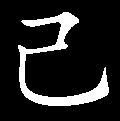
\includegraphics[width=3mm]{../Images/00003}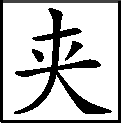
\includegraphics[width=3mm]{../Images/00012}\footnotesize \kaishu 近之淫书满纸伤春,究竟不知伤春原委。看他并不提``伤春''字样,却艳恨}秾{愁,香流满纸矣。}}正悲叹时,忽有一个雀儿飞来,落于枝上乱啼。宝玉又发了呆性,心下想道:``这雀儿必定是杏花正开时他曾来过,今见无花空有子叶,故也乱啼。这声韵必是啼哭之声,可恨公冶长不在眼前,不能问他。但不知明年再发时,这个雀儿可还记得飞到这里来与杏花一会了?''

正胡思间,忽见一股火光从山石那边发出,将雀儿惊飞。宝玉吃一大惊,又听那边有人喊道:``藕官,你要死,怎弄些纸钱进来烧?我回去回奶奶们去,仔细你的肉!''宝玉听了,益发疑惑起来,忙转过山石看时,只见藕官满面泪痕,蹲在那里,手里还拿着火,守着些纸钱灰作悲。宝玉忙问道:``你与谁烧纸钱?快不要在这里烧。你或是为父母兄弟,你告诉我姓名,外头去叫小厮们打了包袱写上名姓去烧。''藕官见了宝玉,只不作一声。宝玉数问不答,忽见一婆子恶恨恨走来拉藕官,口内说道:``我已经回了奶奶们了,奶奶气的了不得。''藕官听了,终是孩气,怕辱没了没脸,便不肯去。婆子道:``我说你们别太兴头过馀了,如今还比你们在外头随心乱闹呢。这是尺寸地方儿。''指宝玉道:``连我们的爷还守规矩呢,你是什么阿物儿,跑来胡闹。怕也不中用,跟我快走罢!''{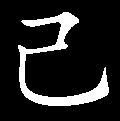
\includegraphics[width=3mm]{../Images/00003}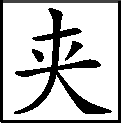
\includegraphics[width=3mm]{../Images/00012}\footnotesize \kaishu 如何?必是含怨之人。又拉上宝玉,画出小人得意来。}宝玉忙道:``他并没烧纸钱,原是林妹妹叫他来烧那烂字纸的。你没看真,反错告了他。''

藕官正没了主意,见了宝玉,也正添了畏惧,忽听他反掩饰,心内转忧成喜,也便硬着口说道:``你很看真是纸钱了么?我烧的是林姑娘写坏了的字纸!''那婆子听如此,亦发狠起来,便弯腰向纸灰中拣那不曾化尽的遗纸,拣了两点在手内,说道:``你还嘴硬,有据有证在这里。我只和你厅上讲去!''说着,拉了袖子,就拽着要走。宝玉忙把藕官拉住,用拄杖敲开那婆子的手,说道:``你只管拿了那个回去。实告诉你:我昨夜作了一个梦,梦见杏花神和我要一挂白纸钱,不可叫本房人烧,要一个生人替我烧了,我的病就好的快。所以我请了白钱,巴巴儿的和林姑娘烦了他来,替我烧了祝赞。原不许一个人知道的,所以我今日才能起来,偏你看见了。我这会子又不好了,都是你冲了!你还要告他去。藕官,只管去,见了他们你就照依我这话说。等老太太回来,我就说他故意来冲神祗,保佑我早死。''藕官听了益发得了主意,反倒拉着婆子要走。那婆子听了这话,忙丢下纸钱,陪笑央告宝玉道:``我原不知道,二爷若回了老太太,我这老婆子岂不完了?我如今回奶奶们去,就说是爷祭神,我看错了。''宝玉道:``你也不许再回去了,我便不说。''婆子道:``我已经回了,叫我来带他,我怎好不回去的。也罢,就说我已经叫到了他,林姑娘叫了去了。''宝玉想了一想,方点头应允。那婆子只得去了。

这里宝玉问他:``到底是为谁烧纸?我想来若是为父母兄弟,你们皆烦人外头烧过了,这里烧这几张,必有私自的情理。''藕官因方才护庇之情感激于衷,便知他是自已一流的人物,便含泪说道:``我这事,除了你屋里的芳官并宝姑娘的蕊官,并没第三个人知道。今日被你遇见,又有这段意思,少不得也告诉了你,只不许再对人言讲。''又哭道:``我也不便和你面说,你只回去背人悄问芳官就知道了。''说毕,佯常而去。

宝玉听了,心下纳闷,{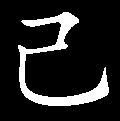
\includegraphics[width=3mm]{../Images/00003}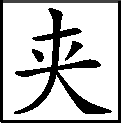
\includegraphics[width=3mm]{../Images/00012}\footnotesize \kaishu 连观书者亦纳闷。}只得踱到潇湘馆,瞧黛玉益发瘦的可怜,问起来,比往日已算大愈了。{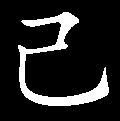
\includegraphics[width=3mm]{../Images/00003}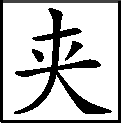
\includegraphics[width=3mm]{../Images/00012}\footnotesize \kaishu 好,若只管病亦不好。}黛玉见他也比先大瘦了,想起往日之事,不免流下泪来,些微谈了谈,便催宝玉去歇息调养。宝玉只得回来。因记挂着要问芳官那原委,偏有湘云香菱来了,正和袭人芳官说笑,不好叫他,恐人又盘诘,只得耐着。

一时芳官又跟了他干娘去洗头。他干娘偏又先叫了他亲女儿洗过了后,才叫芳官洗。芳官见了这般,便说他偏心,``把你女儿剩水给我洗。我一个月的月钱都是你拿着,沾我的光不算,反倒给我剩东剩西的。''他干娘羞愧变成恼,便骂他:``不识抬举的东西!怪不得人人说戏子没一个好缠的。凭你甚么好人,入了这一行,都弄坏了。这一点子屄崽子,也挑幺挑六,咸屄淡舌,咬群的骡子似的!''娘儿两个吵起来。袭人忙打发人去说:``少乱嚷,瞅着老太太不在家,一个个连句安静话也不说。''晴雯因说:``都是芳官不省事,不知狂的什么。也不是会两出戏,倒像杀了贼王、擒了反叛来的。''袭人道:``一个巴掌拍不响,老的也太不公些,小的也太可恶些。''宝玉道:``怨不得芳官。自古说:`物不平则鸣。'{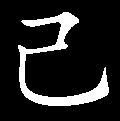
\includegraphics[width=3mm]{../Images/00003}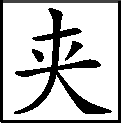
\includegraphics[width=3mm]{../Images/00012}\footnotesize \kaishu 自来经语未遭如是用也。}他少亲失眷的,在这里没人照看,赚了他的钱,又作践他,如何怪得?''因又向袭人道:``他一月多少钱?以后不如你收了过来照管他,岂不省事?''袭人道:``我要照看他那里不照看了,又要他那几个钱才照看他?没的讨人骂去了。''说着,便起身至那屋里取了一瓶花露油并些鸡卵、香皂、头绳之类,叫一个婆子来送给芳官去,叫他另要水自洗,不要吵闹了。他干娘益发羞愧,便说芳官``没良心,花掰我克扣你的钱。''便向他身上拍了几把,芳官便哭起来。宝玉便走出,袭人忙劝:``作什么?我去说他。''晴雯忙先过来,指他干娘说道:``你老人家太不省事。你不给他洗头的东西,我们饶给他东西,你不自臊,还有脸打他。他要还在学里学艺,你也敢打他不成!''那婆子便说:``一日叫娘,终身是母。他排场我,我就打得!''

袭人唤麝月道:``我不会和人拌嘴,晴雯性太急,你快过去震吓他两句。''麝月听了,忙过来说道:``你且别嚷。我且问你,别说我们这一处,你看满园子里,谁在主子屋里教导过女儿的?便是你的亲女儿,既分了房,有了主子,自有主子打得骂得,再者大些的姑娘姐姐们打得骂得,谁许老子娘又半中间管闲事了?都这样管,又要叫他们跟着我们学什么?越老越没了规矩!你见前儿坠儿的娘来吵,你也来跟他学?你们放心,因连日这个病那个病,老太太又不得闲心,所以我没回。等两日消闲了,咱们痛回一回,大家把威风煞一煞儿才好。宝玉才好了些,连我们不敢大声说话,你反打的人狼号鬼叫的。上头能出了几日门,你们就无法无天的,眼睛里没了我们,再两天你们就该打我们了。他不要你这干娘,怕粪草埋了他不成?''宝玉恨的用拄杖敲着门槛子说道:``这些老婆子都是些铁心石头肠子,也是件大奇的事。不能照看,反倒折挫,天长地久,如何是好!''{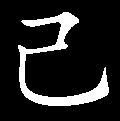
\includegraphics[width=3mm]{../Images/00003}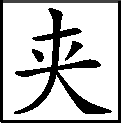
\includegraphics[width=3mm]{../Images/00012}\footnotesize \kaishu 画出宝玉来。}晴雯道:``什么`如何是好',都撵了出去,不要这些中看不中吃的!''那婆子羞愧难当,一言不发。那芳官只穿着海棠红的小棉袄,底下丝绸撒花袷裤,敞着裤腿,{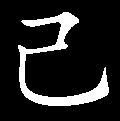
\includegraphics[width=3mm]{../Images/00003}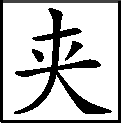
\includegraphics[width=3mm]{../Images/00012}\footnotesize \kaishu 四字奇想,写得纸上跳出一个女优来。}一头乌油似的头发披在脑后,哭的泪人一般。麝月笑道:``把一个莺莺小姐,反弄成拷打红娘了!这会子又不妆扮了,还是这么松怠怠的。''宝玉道:``他这本来面目极好,倒别弄紧衬了。''晴雯过去拉了他,替他洗净了发,用手巾拧干,松松的挽了一个慵妆髻,命他穿了衣服过这边来了。

接着司内厨的婆子来问:``晚饭有了,可送不送?''小丫头听了,进来问袭人。袭人笑道:``方才胡吵了一阵,也没留心听钟几下了。''晴雯道:``那劳什子又不知怎么了,又得去收拾。''说着,便拿过表来瞧了一瞧说:``略等半钟茶的工夫就是了。''小丫头去了。麝月笑道:``提起淘气,芳官也该打几下。昨儿是他摆弄了那坠子半日,就坏了。''说话之间,便将食具打点现成。一时小丫头子捧了盒子进来站住。晴雯麝月揭开看时,还是只四样小菜。晴雯笑道:``已经好了,还不给两样清淡菜吃。这稀饭咸菜闹到多早晚?''一面摆好,一面又看那盒中,却有一碗火腿鲜笋汤,忙端了放在宝玉跟前。宝玉便就桌上喝了一口,{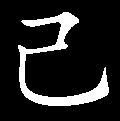
\includegraphics[width=3mm]{../Images/00003}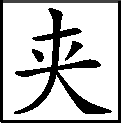
\includegraphics[width=3mm]{../Images/00012}\footnotesize \kaishu 画出病人。}说:``好烫!''袭人笑道:``菩萨,能几日不见荤,馋的这样起来。''一面说,一面忙端起轻轻用口吹。{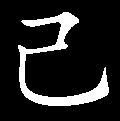
\includegraphics[width=3mm]{../Images/00003}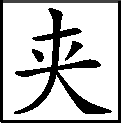
\includegraphics[width=3mm]{../Images/00012}\footnotesize \kaishu 画。}因见芳官在侧,便递与芳官,笑道:``你也学着些伏侍,别一味呆憨呆睡。口劲轻着,别吹上唾沫星儿。''芳官依言果吹了几口,甚妥。

他干娘也忙端饭在门外伺候。向日芳官等一到时原从外边认的,就同往梨香院去了。这干婆子原系荣府三等人物,不过令其与他们浆洗,皆不曾入内答应,故此不知内帏规矩。今亦托赖他们方入园中,随女归房。这婆子先领过麝月的排场,方知了一二分,生恐不令芳官认他做干娘,便有许多失利之处,故心中只要买转他们。今见芳官吹汤,便忙跑进来笑道:``他不老成,仔细打了碗,让我吹罢。''一面说,一面就接。晴雯忙喊:``出去!你让他砸了碗,也轮不到你吹。你什么空儿跑到这里槅子来了?还不出去。''一面又骂小丫头们:``瞎了心的,他不知道,你们也不说给他!''小丫头们都说:``我们撵他,他不出去;说他,他又不信。如今带累我们受气,你可信了?我们到的地方儿,有你到的一半,还有你一半到不去的呢。何况又跑到我们到不去的地方还不算,又去伸手动嘴的了。''一面说,一面推他出去。阶下几个等空盒家伙的婆子见他出来,都笑道:``嫂子也没用镜子照一照,就进去了。''羞的那婆子又恨又气,只得忍耐下去。

芳官吹了几口,宝玉笑道:``好了,仔细伤了气。你尝一口,可好了?''芳官只当是顽话,只是笑看着袭人等。袭人道:``你就尝一口何妨。''晴雯笑道:``你瞧我尝。''说着就喝了一口。芳官见如此,自己也便尝了一口,说:``好了。''递与宝玉。宝玉喝了半碗,吃了几片笋,又吃了半碗粥就罢了。众人拣收出去了。小丫头捧了沐盆,盥漱已毕,袭人等出去吃饭。宝玉使个眼色与芳官,芳官本自伶俐,又学几年戏,何事不知?便装说头疼不吃饭了。袭人道:``既不吃饭,你就在屋里作伴儿,把这粥给你留着,一时饿了再吃。''说着,都去了。

这里宝玉和他只二人,宝玉便将方才从火光发起,如何见了藕官,又如何谎言护庇,又如何藕官叫我问你,从头至尾,细细的告诉他一遍,又问他祭的果系何人。芳官听了,满面含笑,又叹一口气,说道:``这事说来可笑又可叹。''宝玉听了,忙问如何。芳官笑道:``你说他祭的是谁?祭的是死了的菂官。''宝玉道:``这是友谊,也应当的。''芳官笑道:``那里是友谊?他竟是疯傻的想头,说他自己是小生,菂官是小旦,常做夫妻,虽说是假的,每日那些曲文排场,皆是真正温存体贴之事,故此二人就疯了,虽不做戏,寻常饮食起坐,两个人竟是你恩我爱。菂官一死,他哭的死去活来,至今不忘,所以每节烧纸。后来补了蕊官,我们见他一般的温柔体贴,也曾问他得新弃旧的。他说:`这又有个大道理。比如男子丧了妻,或有必当续弦者,也必要续弦为是。便只是不把死的丢过不提,便是情深意重了。若一味因死的不续,孤守一世,妨了大节,也不是理,死者反不安了。'你说可是又疯又呆?说来可是可笑?''宝玉听说了这篇呆话,独合了他的呆性,不觉又是欢喜,又是悲叹,又称奇道绝,说:``天既生这样人,又何用我这须眉浊物玷辱世界。''因又忙拉芳官嘱道:``既如此说,我也有一句话嘱咐他,我若亲对面与他讲未免不便,须得你告诉他。''芳官问何事。宝玉道:``以后断不可烧纸钱。这纸钱原是后人异端,不是孔子的遗训。以后逢时按节,只备一个炉,到日随便焚香,一心诚虔,就可感格了。愚人原不知,无论神佛死人,必要分出等例,各式各例的。殊不知只一`诚心'二字为主。即值仓皇流离之日,虽连香亦无,随便有土有草,只以洁净,便可为祭,不独死者享祭,便是神鬼也来享的。你瞧瞧我那案上,只设一炉,不论日期,时常焚香。他们皆不知原故,我心里却各有所因。随便有新茶便供一钟茶,有新水就供一盏水,或有鲜花,或有鲜果,甚至于荤羹腥菜,只要心诚意洁,便是佛也都可来享,所以说,只在敬不在虚名。以后快命他不可再烧纸。''芳官听了,便答应着。一时吃过饭,便有人回:``老太太、太太回来了------''

{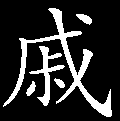
\includegraphics[width=3mm]{../Images/00005}  \kaishu 总评:道理彻上彻下,提笔左潆右拂,浩浩千万言不绝。又恐后人溺词失旨,特自注一句以结穴,曰诚曰信。}

{杏子林对禽惜花一席话,仿佛茂叔庭草不除襟怀。}
